\documentclass[12pt]{article}
\usepackage{xcolor}
\usepackage{amsmath, mathtools}
\usepackage{amsfonts}
\usepackage{amssymb}
\usepackage{graphicx}
\usepackage{colortbl}
\usepackage{xr}
\usepackage{hyperref}
\usepackage{longtable}
\usepackage{xfrac}
\usepackage{tabularx}
\usepackage{float}
\usepackage{siunitx}
\usepackage{booktabs}
\usepackage{caption}
\usepackage{pdflscape}
\usepackage{afterpage}
\usepackage{comment}
\usepackage{hyperref}

\usepackage[round]{natbib}

%\usepackage{refcheck}

\hypersetup{
    bookmarks=true,         % show bookmarks bar?
      colorlinks=true,       % false: boxed links; true: colored links
    linkcolor=red,          % color of internal links (change box color with linkbordercolor)
    citecolor=green,        % color of links to bibliography
    filecolor=magenta,      % color of file links
    urlcolor=cyan           % color of external links
}

%% Comments

\usepackage{color}

\newif\ifcomments\commentstrue

\ifcomments
\newcommand{\authornote}[3]{\textcolor{#1}{[#3 ---#2]}}
\newcommand{\todo}[1]{\textcolor{red}{[TODO: #1]}}
\else
\newcommand{\authornote}[3]{}
\newcommand{\todo}[1]{}
\fi

\newcommand{\wss}[1]{\authornote{blue}{SS}{#1}}
\newcommand{\an}[1]{\authornote{magenta}{Malavika}{#1}}


% For easy change of table widths
\newcommand{\colZwidth}{1.0\textwidth}
\newcommand{\colAwidth}{0.13\textwidth}
\newcommand{\colBwidth}{0.82\textwidth}
\newcommand{\colCwidth}{0.1\textwidth}
\newcommand{\colDwidth}{0.05\textwidth}
\newcommand{\colEwidth}{0.8\textwidth}
\newcommand{\colFwidth}{0.17\textwidth}
\newcommand{\colGwidth}{0.5\textwidth}
\newcommand{\colHwidth}{0.28\textwidth}

% Used so that cross-references have a meaningful prefix
\newcounter{defnum} %Definition Number
\newcommand{\dthedefnum}{GD\thedefnum}
\newcommand{\dref}[1]{GD\ref{#1}}
\newcounter{datadefnum} %Datadefinition Number
\newcommand{\ddthedatadefnum}{DD\thedatadefnum}
\newcommand{\ddref}[1]{DD\ref{#1}}
\newcounter{theorynum} %Theory Number
\newcommand{\tthetheorynum}{T\thetheorynum}
\newcommand{\tref}[1]{T\ref{#1}}
\newcounter{tablenum} %Table Number
\newcommand{\tbthetablenum}{T\thetablenum}
\newcommand{\tbref}[1]{TB\ref{#1}}
\newcounter{assumpnum} %Assumption Number
\newcommand{\atheassumpnum}{P\theassumpnum}
\newcommand{\aref}[1]{A\ref{#1}}
\newcounter{goalnum} %Goal Number
\newcommand{\gthegoalnum}{P\thegoalnum}
\newcommand{\gsref}[1]{GS\ref{#1}}
\newcounter{instnum} %Instance Number
\newcommand{\itheinstnum}{IM\theinstnum}
\newcommand{\iref}[1]{IM\ref{#1}}
\newcounter{reqnum} %Requirement Number
\newcommand{\rthereqnum}{P\thereqnum}
\newcommand{\rref}[1]{R\ref{#1}}
\newcounter{lcnum} %Likely change number
\newcommand{\lthelcnum}{LC\thelcnum}
\newcommand{\lcref}[1]{LC\ref{#1}}

\newcommand{\famname}{CFS} % PUT YOUR PROGRAM NAME HERE

\usepackage{fullpage}

\begin{document}

\title{CFS: Curve Fitting Software} 
\author{Malavika Srinivasan}
\date{\today}

\maketitle

~\newpage

\pagenumbering{roman}

\section{Revision History}

\begin{tabularx}{\textwidth}{p{3cm}p{2cm}X}
\toprule {\bf Date} & {\bf Version} & {\bf Notes}\\
\midrule
Sep 28, 2018 & 1.0 & $0^{th}$ draft by Malavika\\
Oct 2, 2018 & 1.1 & $1^{st}$ draft by Malavika\\
Oct 6, 2018 & 1.2 & $2^{nd}$ draft submitted by Malavika\\
Oct 8, 2018 & 1.2 & $2^{nd}$ Feedback from Robert\\
Oct 10, 2018 & 1.3 & $3^{rd}$ Corrections based on feedback from Robert\\
Oct 11, 2018 & 1.4 & $4^{th}$ Corrections based on feedback from Robert and Dr. Smith\\
Oct 12, 2018 & 1.5 & $5^{th}$ Corrections based on feedback from Robert and Dr.Smith\\
Oct 22, 2018 & 1.6 & $6^{th}$ Corrections based on feedback from Dr.Smith\\
Oct 29, 2018 & 1.7 & $7^{th}$ Corrections after System VnV plan\\
Nov 2, 2018 & 1.8 & $8^{th}$ Corrections based on feedback from Dr.Smith\\
Nov 7, 2018 & 1.9 & $9^{th}$ Corrections based on feedback from Dr.Smith\\
Nov 22, 2018 & 2.0 & $10^{th}$ Corrections based on feedback from Dr.Smith\\
Dec 24, 2018 & 2.1 & $11^{th}$ Final draft for submission.\\
\bottomrule
\end{tabularx}

~\newpage
	
\section{Reference Material}

This section records information for ease of reference. The information includes the units, symbols and abbreviations used in this document.

\subsection{Table of Units}
This library is designed to work for any set of data, irrespective of their units. So, table of units is \textbf{not applicable}. 



\subsection{Table of Symbols}

The table that follows summarizes the symbols used in this document along with
their units. The symbols are listed in alphabetical order.

\renewcommand{\arraystretch}{1.2}
%\noindent \begin{tabularx}{1.0\textwidth}{l l X}
\noindent \begin{longtable*}{l l p{12cm}} \toprule
\textbf{symbol} & \textbf{unit} & \textbf{description}\\
\midrule 
$f$ & & Function\\
$P$ & & Orthogonal matrix\\
$\Phi$ & & Basis function\\
$\Pi$ & & Basis function\\
$\sum_{min}^{max}$& & Summation \\ 
$r$ & & Residual\\
$T$ & & Transpose operation of matrix\\
$v$ & & Basis function\\
\bottomrule
\end{longtable*}


\subsection{Abbreviations and Acronyms}

\renewcommand{\arraystretch}{1.2}
\begin{tabular}{l l} 
  \toprule		
  \textbf{symbol} & \textbf{description}\\
  \midrule 
  A & Assumption\\
  DD & Data Definition\\
  GD & General Definition\\
  GS & Goal Statement\\
  IM & Instance Model\\
  LC & Likely Change\\
  PS & Physical System Description\\
  R & Requirement\\
  %SRS & Software Requirements Specification\\
  CA & Commonality Analysis\\
  \famname & Curve Fitting Software\\
  T & Theoretical Model\\
  \bottomrule
\end{tabular}\\


\newpage

\tableofcontents

~\newpage

\pagenumbering{arabic}

\section{Introduction}

Scientific Computation (SC) is the collection of tools, techniques, and theories that are required to solve problems in the field of science and engineering using computer-based mathematical models. The source data for scientific computation problems are often large sets of data from experiments conducted in a laboratory setup. This large set of data (such as time and temperature) is usually complex to analyze and require segmenting and curve-fitting. Curve fitting is the process of constructing a curve, or mathematical function, that has the best fit to a series of data points possibly subject to constraints.\\

The following section provides an overview of the Commonality Analysis (CA) for a family of softwares developed to fit a set of data points. The developed program will be referred to as Curve Fitting Software(\famname{}). This section explains the purpose of this document, the scope of the family, the organization of the document and the characteristics of intended reader.
 
\wss{80 character width for text in tex file, please}
\ms{Dr.Smith, I already have it set for 80 character width.}
\wss{I don't think you understand what I'm requesting.  I want a hard wrap at 80
  characters.  If you look at the tex file your lines are hundreds of characters
long.  You are probably setting your editor to an 80 character soft wrap.}
\ms{Yes Dr.Smith. I set it to 80 character width soft wrap and now changed it 
to hard wrap. But I don't see places where it is above 80 characters in a line. 
Maybe we can discuss this during tomorrow's meeting.}

\wss{Have a look at your CA.tex file with a web-browser through the GitHub
  interface
  (\url{https://github.com/Malavika-Srinivasan/CAS741/blob/master/docs/SRS/CA.tex}).
You'll see the lines that are longer than 80 characters.}

\subsection{Purpose of Document}
The purpose of this document is to analyze the commonalities and variabilities between the family of softwares produced as part of this library. The commonalities are the elements which are true for each member which is a part of this software family. For instance, curve fitting is common for all the softwares of this family. The variabilities are the elements which may vary between each software member of this family. For instance, the technique used to fit the curve such as interpolation, regression, smoothing are examples of variabilities.


\subsection{Scope of the Family}\label{Scope}
The scope of \famname{} is restricted to finding the best fit parameters of 
linear systems using methods of interpolation and regression discussed in 
chapter $3$ and $7$ of ~\cite{Health1997} . To reduce the complexity of 
\famname{}, we use only polynomials and piecewise polynomials as our basis 
functions for interpolation. In regression, we restrict ourselves to over 
determined linear systems and least squares methods to minimize the residual.
This software will allow only run-time binding for the degree of interpolation 
and regression. There could be also be variabilities associated with the
dimension of the interpolation which could be fixed at build time but this is 
out of scope for \famname{}.\\


 

\subsection{Characteristics of Intended Reader} 
The reader of this document is expected to know the basic concepts of curve fitting. However to obtain a deeper understanding of this document, the reader is expected to be proficient in elementary linear algebra.

\subsection{Organization of Document}
The organization of this document follows the template for a Commonality analysis (CA) for scientific computing software proposed by Dr.Spencer Smith which is based on the SRS template~\cite{SmithEtAl2007},the template for general purpose scientific software~\cite{Smith2006} and the family of material models example~\cite{SmithMcCutchanAndCarette2017}. The sections of this document are grouped into commonalities and variabilities of the \famname{}. The presentation starts with the analyzing commonalities between the softwares of \famname{} which will contain goals, theories,  and definitions which will be common for the family members of \famname{}. Then the variabilities of the family members is presented which will contain the assumptions, instance models and the output. The goal statements are refined to the theoretical models, and theoretical models to the instance models.

\section{General System Description}

This section identifies the interfaces between the system and its environment,
describes the potential user characteristics and lists the potential system
constraints.

\subsection{Potential System Contexts}

Figure~\ref{Fig_SystemContext} shows the system context.  A circle represents an
external entity outside the software, the user in this case.  A rectangle
represents the software system itself (\famname{}).  Arrows are used to show
the data
flow between the system and its environment.

\begin{figure}[h!]
	\begin{center}
		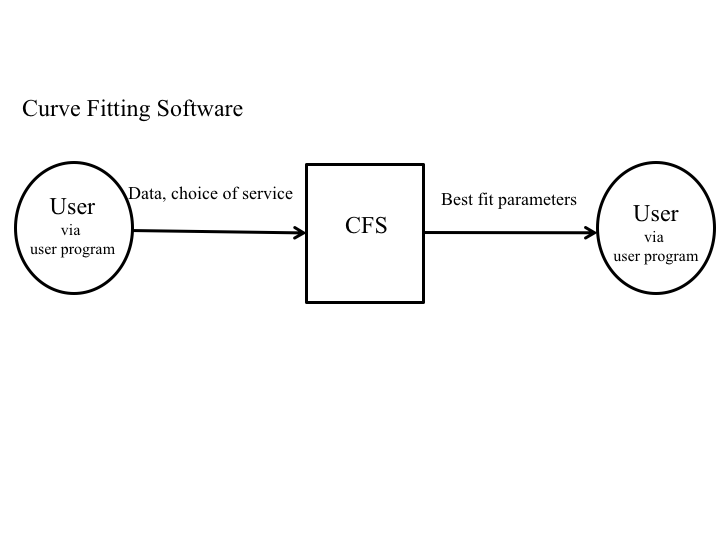
\includegraphics[width=0.6\textwidth]{SystemContextFigure.png}
		\caption{System Context}
		\label{Fig_SystemContext} 
	\end{center}
\end{figure}

\wss{Your figure isn't showing the use of your library correctly.  Your library
  is not used by a User, but by a program.  You can show the user using the
  program, if you like.}
\ms{Change made}

\begin{itemize}
\item User Responsibilities:
\begin{itemize}
\item Enter input data points to be fit.
\item Understand what each point $t_i, y_i$ means with respect to \famname{}.
\item Input whether to use interpolation or regression.
\item Input interpolating method or regression method based on their choice in the previous step. 
\end{itemize}
\item \famname{} Responsibilities:
\begin{itemize}
\item Detect data type mismatch, such as a string of characters instead of a number.
\item Compute best fit parameters.
\end{itemize}
\end{itemize}

\subsection{Potential User Characteristics} \label{SecUserCharacteristics}

The end user of \famname{} should have an understanding of undergraduate Level
regression and interpolation. \wss{You don't need capitals here.}\ms{Changes 
made}

\subsection{Potential System Constraints}

Not Applicable.

\section{Commonalities}

This section presents the common concepts or the information which is true for 
both the methods of curve fitting such as regression and interpolation. The 
background information is available in section \ref{Sec_Background}, followed 
by important terminologies in section \ref{Sec_Terminologies}. The basic 
equations and laws used by \famname{} is geven in sections \ref{sec_gendef} and 
\ref{sec_theoretical}. The data definitions and the goal statements are 
explained in sections \ref{sec_datadef} and \ref{sec_goals}.
\wss{It is good to have text between section headings.  You should put a mini
  roadmap here explaining the contents of this section.}\ms{Makes sense, 
  changes made}

\subsection{Background Overview} \label{Sec_Background}
Curve fitting is the process of constructing a curve, or mathematical function, 
to a series of data points possibly subject to constraints. For regression, the 
best possible fit is chosen and for interpolation,  The figure 
below(\ref{Fig_CurveFitEg}) shows the best fit curve through a series of 
points. \wss{best fit is for regressions.  Interpolation is
  not a best fit.  Interpolation is the only fit that passess exactly through all of the
  data points.}

\begin{figure}[h!]
	\begin{center}
		%rotatebox{-90}
		{
			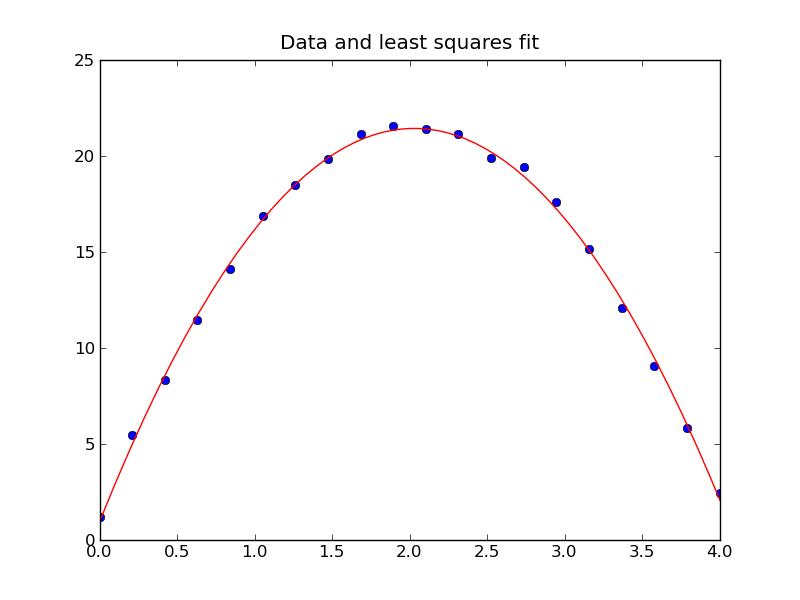
\includegraphics[width=0.5\textwidth]{lstsq11.png}
		}
		\caption{\label{Fig_CurveFitEg} Typical example of a curve fitting process}
	\end{center}
\end{figure}

A fit for the data can be obtained by different methods like interpolation, data smoothing and regression.

\subsubsection{Interpolation}
Interpolation is a process of fitting a function to given data so that the function passes exactly through the data points.

\subsubsection{Smoothing}
Smoothing is a process of creating an approximating function that attempts to capture important patterns in the data, while leaving out noise or other rapid phenomena.

\subsubsection{Regression}
Regression analysis is the process of finding the best fit parameters for a regression model for a given set of data points and thus obtain a curve through a set of data points.

\subsection{Terminology and  Definitions}\label{Sec_Terminologies}

This subsection provides a list of terms that are used in the subsequent
sections and their meaning, with the purpose of reducing ambiguity and making it
easier to correctly understand the requirements:

\begin{itemize}

\item Basis functions: A basis function is an element of a particular basis for a function space. Every continuous function can be represented as a linear combination of basis functions.

\item Transpose: This is a mathematical operation on a matrix by which the rows of a matrix becomes its columns and vice versa.

\item Cholesky Factorization: This is a particular form of this factorization which is commonly used to solve the normal equations that characterize the least squares solution to the overdetermined linear system.

\item Orthogonality: Orthogonality is the generalization of the notion of perpendicularity.

\item Interpolant: An interpolant is a function $L=L(t)$ which agrees with a particular function f at a set of known points $t_0,t_1,t_2,...,t_n$ and which is used to compute values for f(t) at points $t \neq t_i$ where i $=0,1,2,...,n$.

\end{itemize}



\subsection{General Definitions}\label{sec_gendef}

This section collects the equations that will be used in deriving the
data definitions, which in turn will be used to build the instance models.\\

%%%%%%%%%%%%    GD1     %%%%%%%%%%%%%%
~\newline
\noindent
\begin{minipage}{\textwidth}
	\renewcommand*{\arraystretch}{1.5}
	\begin{tabular}{| p{\colAwidth} | p{\colBwidth}|}
		\hline
		\rowcolor[gray]{0.9}
		Number& GD\refstepcounter{defnum}\thedefnum
		\label{GD_CurveFitEq}\\
		\hline
		Label &\bf General form of linear curve fitting\\
		\hline
		SI Units& Not applicable\\
		\hline
		Equation & $f(t) = \sum_{j=1}^{n}x_j \Phi_j (t)$ where $j$ $=
                           1,2,3...m$ \wss{There is no $i$ in this equation.
                           Where is the connection to the data?}\ms{changed i 
                           to j}\\
		\hline
		Description & The above equation gives the general form of linear curve fitting where,
		\begin{itemize}
			\item $(t_i,y_i)$ is the given set of data points, where i $= 1,2, 3...m$.
			\item The functions $\Phi(t), \Phi_1(t), ... \Phi_n(t)$ are basis functions whose linear combination yields the curve fitting function $f$.
			\item $x_j$ is the parameters of the best fit.
		\end{itemize}\\
		\hline
		Source & ~\cite{Health1997}\\
		\hline
		
		Ref.\ By &\tref{T_Interpolation}, \tref{T_LinearRegression}, \iref{IM_Polynomial},\iref{IM_Piecewise}, \iref{IM_Monomial}, \iref{IM_Lagrange}, \iref{IM_Newton}, \iref{IM_HermiteCubic} and \iref{IM_BSpline}\\
		\hline
	\end{tabular}
\end{minipage}\\

%%%%%%%%%%%%%%%%%%%%%%%%%%%%%%%%%%%%%%%%%%%%%%%%%%%%%%%%%%%%%5
~\newline
\noindent
\begin{minipage}{\textwidth}
	\renewcommand*{\arraystretch}{1.5}
	\begin{tabular}{| p{\colAwidth} | p{\colBwidth}|}
		\hline
		\rowcolor[gray]{0.9}
		Number& GD\refstepcounter{defnum}\thedefnum
		\label{GD_OverdetLinearSys}\\
		\hline
		SI Units& Not applicable\\
		\hline
		Label & \bf Overdetermined Linear Systems\\
		\hline
		Equation
		& For a given set of n data points, $(t_i,y_i)$ i $= {1,2,...n}$
                  represented in matrix form $Ax = y$ as in
                  \tref{T_LinearEqMatrix}, where $A$ is an $m \times n$ matrix with $m > n$ which means there are more equations than unknowns. \\		
		& A solution to the system $x$ can be computed such that the residual vector,
		\begin{equation*}
		r = y - Ax
		\end{equation*} is small. 
		where $i = 1,2,3 ....n$.\\
		\hline
		
		Description 
		& The symbols used in this equation are .\\
		& $(t_i,y_i)$ is the given input data.\\
		& To find a solution to this problem we use least squares method.(\tref{T_LeastSquares})\\
		\hline
		
		Sources& Some related information is available at:
		\url{https://s-mat-pcs.oulu.fi/~mpa/matreng/ematr5_5.htm}\\
		\hline
		Ref.\ By & \tref{T_LinearEqMatrix}, \iref{IM_NormalEquations}, \iref{IM_AugmentedSystem}, \iref{IM_OrthogonalTransformation}\\
		\hline
	\end{tabular}
\end{minipage}\\

\subsection{Theoretical Models} \label{sec_theoretical}

This section focuses on the general equations that \famname{} is based on.
~\newline

%%%%%%%%%%%%%%%%%%%%%%%%%%%%        Ax = y      %%%%%%%%%%%%%%%%%%%%%%%%%%%%%%

\noindent
\begin{minipage}{\textwidth}
	\renewcommand*{\arraystretch}{1.5}
	\begin{tabular}{| p{\colAwidth} | p{\colBwidth}|}
		\hline
		\rowcolor[gray]{0.9}
		Number& T\refstepcounter{theorynum}\thetheorynum \label{T_LinearEqMatrix}\\
		\hline
		Label&\bf Matrix-Vector notation for a system of linear equations.\\
		\hline
		Equation& \begin{equation*}
		Ax = y
		\end{equation*} \\
		\hline
		Description & The above equation gives the general form of system of linear equations in matrix vector notation where,\\
		& $A$ is a $m \times n$ matrix\\
		& $y$ is an $m$-vector\\
		& $x$ is an $n$-vector\\
		\hline
		Source & ~\cite{Health1997}\\
		
		\hline
		Ref.\ By & \iref{IM_Monomial}, \iref{IM_Lagrange}, \iref{IM_Newton}, \iref{IM_HermiteCubic}, \iref{IM_NormalEquations}, \iref{IM_AugmentedSystem} and \iref{IM_OrthogonalTransformation}\\
		\hline
	\end{tabular}
\end{minipage}\\
~\newline

%%%%%%%%%%%%%%%%%%%%%%%%%%%%        Least squares     %%%%%%%%%%%%%%%%%%%%%%%%%%
~\newline
\noindent
\begin{minipage}{\textwidth}
	\renewcommand*{\arraystretch}{1.5}
	\begin{tabular}{| p{\colAwidth} | p{\colBwidth}|}
		\hline
		\rowcolor[gray]{0.9}
		Number& T\refstepcounter{theorynum}\thetheorynum \label{T_LeastSquares}\\
		\hline
		Label&\bf Least Squares method.\\
		\hline
		Equation& For a given overdetermined system of equations represented in 
		matrix form as in \tref{T_LinearEqMatrix}, a best fit solution $x$ is 
		found such that, the square of the difference between the actual and 
		expected output is minimum. This is mathematically represented as shown 
		below.
		\begin{equation*}
		\min_{x}\sum_{i=1}^{m} (y_i - f(t_i,x)) ^2
		\end{equation*} \\
		\hline
		Description & The above mathematical expression gives the definition of 
		best fit solution in least squares method.\\
		& A is a $m$ X $n$ matrix\\
		& y is a m-vector\\
		& x is an n-vector\\
		\hline
		Source & ~\cite{Health1997}\\
		
		\hline
		Ref.\ By &\iref{IM_NormalEquations}, \iref{IM_AugmentedSystem} and \iref{IM_OrthogonalTransformation}\\
		\hline
	\end{tabular}
\end{minipage}\\
\wss{What is the connection between the equation and the description?  Is this a
  copy and paste error?}\ms{Yes, I guess it should say mathematical expression 
  instead of equation. Changed}
~\newline

%%%%%%%%%%%%%%%%%%%%%% T_Interpolation  %%%%%%%%%%%%%%%%%%%%%%%%

~\newline
\noindent
\begin{minipage}{\textwidth}
	\renewcommand*{\arraystretch}{1.5}
	\begin{tabular}{| p{\colAwidth} | p{\colBwidth}|}
		\hline
		\rowcolor[gray]{0.9}
		Number& T\refstepcounter{theorynum}\thetheorynum \label{T_Interpolation}\\
		\hline
		Label&\bf General form of Interpolation\\
		\hline
		Equation&  $f(t_i) = \sum_{j=1}^{n}x_j \Phi_j (t) = y_i$ where i $= 1,2,3...m$\\
		\hline
		Description & 
		The above equation gives the general form of interpolating function where,
		\begin{itemize}
			\item $(t_i,y_i)$ is the given set of data points, where i $= 1,2, 3...m$.
			\item The functions $\Phi(t), \Phi_1(t), ... \Phi_n(t)$ are basis functions whose linear combination yields the interpolating function $f$ whose value at a given $t_i$ is $y_i$.
			\item $x_j$ is the parameters of the curve fit. \wss{The
                            terminology best fit doesn't make sense here.  Curve
                            fit would be fine.}\ms{changed the terminology}
			\item $y_i$ is the given data point at $t_i$.
		\end{itemize}\\
		\hline
		Source & ~\cite{Health1997}\\
		
		\hline
		Ref.\ By & \dref{GD_CurveFitEq}, \iref{IM_Polynomial}, \iref{IM_Piecewise}, \iref{IM_Monomial}, \iref{IM_Lagrange}, \iref{IM_Newton}, \iref{IM_HermiteCubic}, \iref{IM_NormalEquations}, \iref{IM_AugmentedSystem} and \iref{IM_OrthogonalTransformation}\\
		\hline
	\end{tabular}
\end{minipage}\\
%%%%%%%%%%%%%%%%%%%%%%     Least Squares %%%%%%%%%%%%%%%%%%%%%%%%%%%%%%%%
~\newline
\noindent
\begin{minipage}{\textwidth}
	\renewcommand*{\arraystretch}{1.5}
	\begin{tabular}{| p{\colAwidth} | p{\colBwidth}|}
		\hline
		\rowcolor[gray]{0.9}
		Number& T\refstepcounter{theorynum}\thetheorynum \label{T_LinearRegression}\\
		\hline
		Label&\bf General form of Linear Regression using Least squares method and best fit in least squares. \\
		\hline
		Equation&  For i $= 1,2,3...m$, general form of regression is given by
		\begin{equation*}
		f(t_i) = \sum_{j=1}^{n}x_j \Phi_j (t)	
		\end{equation*} 
		~\newline
		Since we deal with only linear problems(\ref{Scope}), $\Phi_j$ depend only on $t$. Hence $f(t_i,x) $ can be expressed as,
		\begin{equation*}
		f(t_i) = x_1 + x_2 t + x_3 t^{2} + ... + x_n t^{n-1}.
		\end{equation*}
		~\newline
		where $x_i$ is the parameters of the curve fit, such that the Least 
		squares as defined \tref{T_LeastSquares} is minimum. \wss{I don't see 
		the connection to T2 as T2 is currently written.}\ms{I can see the 
		disconnection. I changed it now. Can you please review this?}
                          \wss{You are on the right track now.  There are still
                          some issues with attention to detail, like $f$ is
                          sometimes a function of one variable and sometimes a
                          function of two variables, but this is now on the
                          right track.}\ms{Corrected.}\\ 
		\hline
		Description & 
		The above equation gives the general form of linear regression function and the definition of best fit in least squares method.\\
		
		&$(t_i,y_i)$ is the given set of data points, where i $= 1,2, 3...m$.\\
		&The functions $\Phi(t), \Phi_1(t), ... \Phi_n(t)$ are basis functions whose linear combination yields the function $f$ whose value at any $t$ is the best fit to the given data.\\
		&$x_j$ is the parameters of the best fit.\\
		\hline
		Source & ~\cite{Health1997}\\
		
		\hline
		Ref.\ By & \dref{GD_CurveFitEq}, \iref{IM_NormalEquations}, \iref{IM_AugmentedSystem} and \iref{IM_OrthogonalTransformation}\\
		\hline
	\end{tabular}
\end{minipage}\\

~\newline



\subsection{Data Definitions} \label{sec_datadef}

This section collects and defines all the data needed to build the instance
models. The dimension of each quantity is also given. 

~\newline
\noindent
\begin{minipage}{\textwidth}
\renewcommand*{\arraystretch}{1.5}
\begin{tabular}{| p{\colAwidth} | p{\colBwidth}|}
\hline
\rowcolor[gray]{0.9}
Number
& DD\refstepcounter{datadefnum}\thedatadefnum \label{DD_Monomial}\\
\hline

Label
& \bf Data definitions of monomial interpolation method.\\
\hline

Symbol 
&$\Phi$, $A$ and $y$.\\
\hline

SI Units 
& Not applicable\\
\hline

Equation
	&For the given set of data $(t_i, y_i)$ where j $= {1,2,...n}$, the below equation gives the basis functions.
\begin{equation*}
\Phi_j (t) = t^{j-1} 
\end{equation*}
\\
&The matrix A and y is given by,
\begin{equation*}
A = \begin{bmatrix}
1 & t_{1} & t_{1} ^2 & \dots & t_{1} ^{n-1} \\
1 & t_{2} & t_{2} ^2 & \dots & t_{2} ^{n-1} \\
\vdots & \vdots & \vdots & \vdots \\
1 & t_{n} & t_{n} ^2 & \dots & t_{n} ^{n-1} \\
\end{bmatrix}
\end{equation*}
\begin{equation*}
y = \begin{bmatrix}
y_1  \\
y_2 \\
\vdots \\
y_n \\
\end{bmatrix} 
\end{equation*} \\
\hline
Description 
&To provide the basis functions and matrices necessary for monomial interpolation \iref{IM_Monomial}.\\
& The symbols used in the above equation are $\Phi_j(t)$ which represents the basis function at any t in the data $(t_i, y_i)$.\\
&A and y are matrices representing the system of equations through the given set of data points.\\
\hline

Sources
& ~\cite{Health1997}\\
\hline

Ref.\ By 
& \iref{IM_Monomial}\\
\hline

\end{tabular}
\end{minipage}\\
%%%%%%%%%%%%%%%%%%%%%%%%%%%%%%%     DD_Lagrange   %%%%%%%%%%%%%%%%%%%%%%%%

~\newline

\noindent
\begin{minipage}{\textwidth}
	\renewcommand*{\arraystretch}{1.5}
	\begin{tabular}{| p{\colAwidth} | p{\colBwidth}|}
		\hline
		\rowcolor[gray]{0.9}
		Number
		& DD\refstepcounter{datadefnum}\thedatadefnum \label{DD_Lagrange}\\
		\hline
		
		Label
		& \bf Data definitions of Lagrange's interpolation method.\\
		\hline
		
		Symbol 
		&$l$, $A$ and $y$.\\
		\hline
		
		SI Units 
		& Not applicable\\
		\hline
		
		Equation
		&For the given set of data $(t_i, y_i)$ where j $= {1,2,...n}$, the below equation gives the basis functions.
		\begin{equation*}
		l_j (t) =  \frac{ \Pi _{k=1, k\neq j} ^n (t - t_k)} {\Pi _{k=1,k \neq j} ^ n (t_j - t_k)} = \frac{(t - t_1)}{(t_j - t_1)}...\frac{(t - t_{j-1})}{(t_j - t_{j-1})}\frac{(t - t_{j+1})}{(t_j - t_{j+1})}... \frac{(t - t_n)}{(t_j - t_n)}
		\end{equation*}
		\\
		&The matrix A(Identity matrix) and y is given by,
		\begin{equation*}
		A = \begin{bmatrix}
		1 & 0 & 0 & \dots & 0 \\
		0 & 1 & 0 & \dots & 0 \\
		\vdots & \vdots & \vdots & \vdots \\
		0 & 0 & 0 & \dots & 1 \\
		\end{bmatrix}
		\end{equation*}
		\begin{equation*}
		y = \begin{bmatrix}
		y_1  \\
		y_2 \\
		\vdots \\
		y_n \\
		\end{bmatrix}
		\end{equation*} \\
		\hline
Description 
&To provide the basis functions and matrices necessary for lagrange's interpolation \iref{IM_Lagrange}.\\
& The symbols used in the above equation are $l_j(t)$ which represents the basis function at any t in the data $(t_i, y_i)$.\\
&A and y are matrices representing the system of equations through the given set of data points.\\
\hline

Sources
& ~\cite{Health1997}\\
\hline

Ref.\ By 
& \iref{IM_Lagrange}\\
\hline

\end{tabular}
\end{minipage}\\

%%%%%%%%%%%%%%%%%%%%%%    DD_Newton      %%%%%%%%%%%%%%%%%%%%%%%%%%%


~\newline
\noindent
\begin{minipage}{\textwidth}
	\renewcommand*{\arraystretch}{1.5}
	\begin{tabular}{| p{\colAwidth} | p{\colBwidth}|}
		\hline
		\rowcolor[gray]{0.9}
		Number
		& DD\refstepcounter{datadefnum}\thedatadefnum \label{DD_Newton}\\
		\hline
		
		Label
		& \bf Data definitions of Newton interpolation method.\\
		\hline
		
		Symbol 
		&$\pi$, $A$ and $y$.\\
		\hline
		
		SI Units 
		& Not applicable\\
		\hline
		
		Equation
		&For the given set of data $(t_i, y_i)$ where j $= {1,2,...n}$, the below equation gives the basis functions.
		\begin{equation*}
		\pi(t) = \Pi_{k=1}^{j-1} (t - t_k)  
		\end{equation*}
		When the limits make it vacuous, the product is taken to be 1.\\
		& Also, $\pi_j (t) = 0$ for $i < j$.
		\\
		&The matrix A and y is given by,
		
		A is a lower triangular as $\pi_j (t) = 0$ for $i < j$ with its entries defined by $a_{ij} = \pi_j (t_i)$
		\begin{equation*}
		A = \begin{bmatrix}
		\pi_0 (t_0) & 0           & 0            & \dots         & 0 \\
		
		\pi_0 (t_1) & \pi_1 (t_1) & 0            & \dots         & 0 \\
		\vdots      & \vdots      & \vdots       &\ddots         & 0 \\
		\pi_0 (t_n) & \pi_1 (t_n) & \pi_2 (t_n)  & \dots         & \pi_n (t_n) \\
		\end{bmatrix}
		\end{equation*}
		\begin{equation*}
		y = \begin{bmatrix}
		y_1  \\
		y_2 \\
		\vdots \\
		y_n \\
		\end{bmatrix} 
		\end{equation*} \\
		\hline
		
		Description 
		&To provide the basis functions and matrices necessary for Newton's interpolation \iref{IM_Newton}.\\
		& The symbols used in the above equation are $\pi_j(t)$ which represents the basis function at any t in the data $(t_i, y_i)$.\\
		&A and y are matrices representing the system of equations through the given set of data points.\\
		\hline
		
		
		Sources
		& ~\cite{Health1997}\\
		\hline
		
		Ref.\ By 
		& \iref{IM_Newton}\\
		\hline
		
	\end{tabular}
\end{minipage}\\
%%%%%%%%%%%%%%%%%%%%%%%%%%%%%%%     DD_HermiteCubic   %%%%%%%%%%%%%%%%%%%%%%%%

~\newline
\noindent
\begin{minipage}{\textwidth}
	\renewcommand*{\arraystretch}{1.5}
	\begin{tabular}{| p{\colAwidth} | p{\colBwidth}|}
		\hline
		\rowcolor[gray]{0.9}
		Number
		& DD\refstepcounter{datadefnum}\thedatadefnum \label{DD_HermiteCubic}\\
		\hline
		
		Label
		& \bf Data definitions of Hermite Cubic interpolation method.\\
		\hline
		
		Symbol 
		&$A$ and $y$.\\
		\hline
		
		SI Units 
		& Not applicable\\
		\hline
		
		Equation
		&The matrix A and y is given by,\\
		&$
		A = \begin{bmatrix}
		1          & t_0       & t_0 ^{2}         & t_0 ^{3}         \\
		\vdots     & \vdots    & \vdots           & \vdots            \\
		1          & t_n       & t_n ^{2}         & t_n ^{3}          \\
		0          & 1         & 2 t_0            & 3 t_0 ^{2}         \\
		\vdots     & \vdots    & \vdots           & \vdots            \\
		0          & 1         & 2 t_n            & 3 t_n ^{2}          \\
		0          & 0         & 2                & 6 t_0              \\
		\vdots     & \vdots    & \vdots           & \vdots            \\
		0          & 0         & 2                & 6 t_n           \\
		0          & 0         & 0                & 6                 \\
		\vdots     & \vdots    & \vdots           & \vdots            \\
		0          & 0         & 0                & 6               \\
		\end{bmatrix}$ and $y = \begin{bmatrix}
		y_0  \\
		\vdots \\
		y_0 ^{(1)} \\
		y_1 ^{(1)} \\
		\vdots \\
		y_n ^{(1)} \\
		y_1 ^{(2)} \\
		\vdots \\
		y_n ^{(2)} \\  
		y_1 ^{(3)} \\
		\vdots \\
		y_n ^{(3)} \\ 
		\end{bmatrix}
		$ \\
		\hline
		Description 
		&To provide the matrices necessary for Hermite cubic interpolation \iref{IM_HermiteCubic}.\\
		&A and y are matrices representing the system of equations through the given set of data points.\\
		\hline
		
		Sources
		& Some related information can be obtained at: \url{https://coast.nd.edu/jjwteach/www/www/30125/pdfnotes/lecture5_9v14.pdf}\\
		\hline
		
		Ref.\ By 
		& \iref{IM_HermiteCubic}\\
		\hline
		
	\end{tabular}
\end{minipage}\\


%%%%%%%%%%%%%%%%%%%%%%%%%%%%%%%     DD_BSpline  %%%%%%%%%%%%%%%%%%%%%%%%

~\newline
\noindent
\begin{minipage}{\textwidth}
	\renewcommand*{\arraystretch}{1.5}
	\begin{tabular}{| p{\colAwidth} | p{\colBwidth}|}
		\hline
		\rowcolor[gray]{0.9}
		Number
		& DD\refstepcounter{datadefnum}\thedatadefnum \label{DD_B-Spline}\\
		\hline
		
		Label
		& \bf Data definitions of B-Spline interpolation.\\
		\hline
		
		Symbol 
		&$v ^{k} _i (t)$\\
		\hline
		
		SI Units 
		& Not applicable\\
		\hline
		
		Equation
		&The basis function for B-Spline is given by:
		\begin{equation*}
		v_i ^k = \frac{t-t_i}{t_{i+k} - t_i}
		\end{equation*}
		\\
		\hline
		
		Description 
		&To provide the basis function for BSpline interpolation \iref{IM_BSpline}.\\
		\hline
		
		Sources
		& ~\cite{Health1997}\\
		\hline
		
		Ref.\ By 
		& \iref{IM_BSpline}\\
		\hline
		
	\end{tabular}
\end{minipage}\\

%%%%%%%%%%%%%%%%%%%%%%%%%%%%%%%     DD_Matrix Transpose %%%%%%%%%%%%%%%%%%%%%%%
~\newline
\noindent
\begin{minipage}{\textwidth}
	\renewcommand*{\arraystretch}{1.5}
	\begin{tabular}{| p{\colAwidth} | p{\colBwidth}|}
		\hline
		\rowcolor[gray]{0.9}
		Number
		& DD\refstepcounter{datadefnum}\thedatadefnum \label{DD_MatrixTranspose}\\
		\hline
		
		Label
		& \bf Matrix Transpose\\
		\hline
		
		Symbol 
		&$A^{T}$\\
		\hline
		
		SI Units 
		& Not applicable\\
		\hline
		
		Equation
		&
		\begin{equation*}
		[A^{T}]_{ij} = [A]_{ji}
		\end{equation*}\\
		\hline
		
		Description 
		&The symbols used in the equations are,\\ 
		& $i, j$ represents the rows and columns of a matrix.\\
		& T represents the transpose operation of a matrix.\\
		
		\hline
		
		Sources
		& ~\cite{Health1997}\\
		\hline
		
		Ref.\ By 
		& \iref{IM_NormalEquations}, \iref{IM_AugmentedSystem}\\
		\hline
		
	\end{tabular}
\end{minipage}\\
  
%%%%%%%%%%%%%%%%%%%%%%%%%%%%%%%     DD_NormalEquations  %%%%%%%%%%%%%%%%%%%%%%%%
~\newline
\noindent
\begin{minipage}{\textwidth}
	\renewcommand*{\arraystretch}{1.5}
	\begin{tabular}{| p{\colAwidth} | p{\colBwidth}|}
		\hline
		\rowcolor[gray]{0.9}
		Number
		& DD\refstepcounter{datadefnum}\thedatadefnum \label{DD_NormalEquations}\\
		\hline
		
		Label
		& \bf Data definitions of Regression using Normal Equations.\\
		\hline
		
		Symbol 
		&$A^{T} A$\\
		\hline
		
		SI Units 
		& Not applicable\\
		\hline
		
		Equation
		&
		\begin{equation*}
		A^{T} A = L L^{T}
		\end{equation*}
		\begin{equation*}
		[A^{T}]_{ij} = [A]_{ji}
		\end{equation*}\\
		\hline
		
		Description 
		&The symbols used in the equations are,\\ 
		& $L$ represents the lower triangular matrix for Cholesky Factorization.\\
		& $i, j$ represents the rows and columns of a matrix.\\
		& T represents the transpose operation of a matrix.\\
		
		\hline
		
		Sources
		& ~\cite{Health1997}\\
		\hline
		
		Ref.\ By 
		& \iref{IM_NormalEquations}\\
		\hline
		
	\end{tabular}
\end{minipage}\\


%%%%%%%%%%%%%%%%%%%%%%%%%%%%%%%     DD_Orthogonality Matrix %%%%%%%%%%%%%%%%%%
~\newline
\noindent
\begin{minipage}{\textwidth}
	\renewcommand*{\arraystretch}{1.5}
	\begin{tabular}{| p{\colAwidth} | p{\colBwidth}|}
		\hline
		\rowcolor[gray]{0.9}
		Number
		& DD\refstepcounter{datadefnum}\thedatadefnum \label{DD_OrthogonalityMatrix}\\
		\hline
		
		Label
		& \bf Orthogonality Matrix\\
		\hline
		
		Symbol 
		&$P$\\
		\hline
		
		SI Units 
		& Not applicable\\
		\hline
		
		Equation
		&\begin{equation*}
		P =  (\frac{A A^{T}}{A^{T} A} )  y
		\end{equation*}\\
		\hline
		
		Description 
		&The symbols used in the equations are,\\ 
		& $P$ represents the orthogonal matrix of A.\\
		& T represents the transpose operation of a matrix.\\
		
		\hline
		
		Sources
		& Some related information is given at: \url{http://uspas.fnal.gov/materials/05UCB/4_LSQ.pdf}\\
		\hline
		
		Ref.\ By 
		& \iref{IM_OrthogonalTransformation}\\
		\hline
		
	\end{tabular}
\end{minipage}\\



\subsection{Goal Statements}\label{sec_goals}

\noindent Given the set of data points, the choice of software from \famname{} and the variabilities of the software the \famname{} should:

\begin{itemize}

\item[GS\refstepcounter{goalnum}\thegoalnum \label{G_bestfit}:] compute the parameters of the curve which is the best possible fit through the set of data points.

\end{itemize}



\section{Variabilities}

\subsection{Assumptions}

\begin{itemize}

\item[A\refstepcounter{assumpnum}\theassumpnum \label{A_data}:] For the given `n' number of data points $(t_i,y_i)$ where i $= 0,1,2,...n$, n $\geq 2$.(\rref{R_IInputs})
\item[A\refstepcounter{assumpnum}\theassumpnum \label{A_dataConstraint}:] For the given `n' number of data points $(t_i,y_i)$ where i $= 0,1,2,...n$, $t_i < t_{i+1}$.(\iref{IM_HermiteCubic},\iref{IM_BSpline})
\item[A\refstepcounter{assumpnum}\theassumpnum \label{A_Interpolation}:] For the given set of data points $(t_i,y_i)$ where i $= 0,1,2,...n$,  there exists an interpolant.(\iref{IM_Polynomial}, \iref{IM_Piecewise}, \iref{IM_Monomial}, \iref{IM_Lagrange}, \iref{IM_Newton}, \iref{IM_HermiteCubic} and \iref{IM_BSpline}).

\item[A\refstepcounter{assumpnum}\theassumpnum \label{A_Regression}:] For the given set of data points $(t_i,y_i)$, there exists a least squares solution.(\iref{IM_NormalEquations}, \iref{IM_AugmentedSystem} and \iref{IM_OrthogonalTransformation})
\item[A\refstepcounter{assumpnum}\theassumpnum \label{A_BSplines}:] We assume only linear basis functions for B-Splines. (\iref{IM_BSpline}) 


\end{itemize}

\subsection{Calculation} \label{sec_Calculation}


%%%%%%%%%%%%%%%%%%%%%%%%%%%%%%%%%%%%%%%%%%%%

\subsubsection{Instance Model} \label{PolynomialInterpolation}    

This section transforms the goal of \famname{} defined in the 
Section~\ref{sec_goals} into one which is expressed in mathematical terms. It 
uses concrete symbols defined in Section~\ref{sec_datadef} to replace the 
abstract symbols in the models identified in the Sections~\ref{sec_theoretical} 
and~\ref{sec_gendef}. All the instance models presented below are based on 
system of equations which is solved using matrices.

~\newline
\noindent
\begin{minipage}{\textwidth}
	\renewcommand*{\arraystretch}{1.5}
	\begin{tabular}{| p{\colAwidth} | p{\colBwidth}|}
		\hline
		\rowcolor[gray]{0.9}
		Number
		& IM\refstepcounter{instnum}\theinstnum \label{IM_Polynomial}\\
		\hline
		
		Label
		& \bf Polynomial Interpolation\\
		\hline
		
		Input
		& A set of n data points, $(t_i,y_i)$ i $= {1,2,...n}$\\		
		\hline
		
		Output& $P_{n-1}(t)$ is a polynomial of degree atmost $n-1$ such that 
		\begin{equation*}
		P_{n-1}(t_i) = y_i
		\end{equation*}
		where $i = 1,2,3 ....n$
		\\
		\hline
		
		Description 
		& The symbols used in this equation are $P_{n-1}$ which represents the polynomial of degree at the most $n-1$.\\
		& $(t_i,y_i)$ is the given input data where no two $t_i$ are the same.\\
		&Polynomial interpolation has different variabilities which are
                  discussed in separate instance models \iref{IM_Monomial}, 
                  \iref{IM_Lagrange} and \iref{IM_Newton}. 
                  \wss{You should make an explicit connection.}\ms{Changes 
                  made}\\
		\hline
		
		Sources
		& Some related information is available at~\cite{Health1997}\\
		\hline
		Ref.\ By & \tref{T_Interpolation}, \iref{IM_Monomial}, \iref{IM_Lagrange}, \iref{IM_Newton}, and \rref{R_Imethod}\\
		\hline
	\end{tabular}
\end{minipage}\\

%%%%%%%%%%%%%%%%%%%%%%%%%%%%%%%%%%%%%%%%%%%%%%%%%%%%%%%%%%%%%5

~\newline
\noindent
\begin{minipage}{\textwidth}
	\renewcommand*{\arraystretch}{1.5}
	\begin{tabular}{| p{\colAwidth} | p{\colBwidth}|}
		\hline
		\rowcolor[gray]{0.9}
		Number
		& IM\refstepcounter{instnum}\theinstnum \label{IM_Piecewise}\\
		\hline
		
		Label
		& \bf Piecewise Interpolation\\
		\hline
		
		Input
		& A set of n data points, $(t_i,y_i)$ i $= {1,2,...n}$ where $t_{i+1} > 
		t_i$.\\		
		\hline
		
		Output& $P(t) = L_i (t)$ is a piecewise linear function where
                        $L_i$ is given \wss{spell check}\ms{changed} by the 
                        following equation. 
		\begin{equation*}
		L_i,i+1 (t) = p(x) 
		\end{equation*}
		for each interval $[t_i,t_{i+1})$, where $i = 1,2,3 ....n$. The degree 
		of the polynomial can be varied as per requirement in each interval. \\
		
		\hline
		
		Description 
		& The symbols used in this equation are $P(t)$ which represents the piecewise polynomial of degree $1$.\\
		& $(t_i,y_i)$ is the given input data where no two $t_i$ are the same.\\
		&Piecewise interpolation has different variabilities which are 
		discussed as separate instance models.\\
		& By default, the interval is same as $t$ array. So, the interval in an 
		array t = [$t_0, t_1, t_2, t_3$] is [$t_0,t1$), [$t1, t2$) and [$t_2, 
		t3$].\\
		\hline
		
		Sources& Some related information is available at:
		 \url{http://www.math.umd.edu/~petersd/460/spline.pdf}\\
		\hline
		Ref.\ By & \tref{T_Interpolation}, \iref{IM_HermiteCubic}, \iref{IM_BSpline} and
		\rref{R_Imethod}\\
		\hline
	\end{tabular}
\end{minipage}\\





%%%%%%%%%%%%%%%%%%%%%%%%%%%%%%%%%%%%%

~\newline
\noindent
\begin{minipage}{\textwidth}
	\renewcommand*{\arraystretch}{1.5}
	\begin{tabular}{| p{\colAwidth} | p{\colBwidth}|}
		\hline
		\rowcolor[gray]{0.9}
		Number
		& IM\refstepcounter{instnum}\theinstnum \label{IM_Monomial}\\
		\hline
		
		Label
		& \bf Monomial Interpolation\\
		\hline
		
		Input
		& $(t_i,y_i)$ i $= {1,2,...n}$\\
		& see~\ddref{DD_Monomial}, from which the basis function of the monomial interpolation is obtained.\\
		& see~\ddref{DD_Monomial}, from which the definition of matrix A and b are obtained.\\
		\hline
		
		Output
		&Find $P_{n-1}(t)$ such that for the given input $(t_i,y_i)$,
		\begin{equation*}
		P_{n-1}(t_i) = x_1 + x_2 t_i + x_3 t_i ^2 + x_4 t_i ^3 + ... x_n t_i ^{n-1} = y_i 
		\end{equation*}
		Where $x_1, x_2, x_3 ... x_n$ can be obtained by representing the above system of linear equations in matrix form $Ax = b$ as in \tref{T_LinearEqMatrix} and solving for x using the equation below.
		\begin{equation*}
		Ax = \begin{bmatrix}
		1 & t_{1} & t_{1} ^2 & \dots & t_{1} ^{n-1} \\
		1 & t_{2} & t_{2} ^2 & \dots & t_{2} ^{n-1} \\
		\vdots & \vdots & \vdots & \vdots \\
		1 & t_{n} & t_{n} ^2 & \dots & t_{n} ^{n-1} \\
		\end{bmatrix}
		\begin{bmatrix}
		x_1  \\
		x_2 \\
		\vdots \\
		x_n \\
		\end{bmatrix} = 
		\begin{bmatrix}
		y_1  \\
		y_2 \\
		\vdots \\
		y_n \\
		\end{bmatrix} = y
		\end{equation*}\\ 
	
		
		\hline
		Description & To determine the interpolating polynomial $p_{n-1}$ for a given set of input points.\\
		& The symbols used in this equation are $P_{n-1}$ which represents the polynomial of degree at the most $n-1$.\\
		& $x_1, x_2 ... x_n$ are best fit parameters.\\
		\hline
		
		Sources& Some related information is available at:~\cite{Health1997}\\
		\hline
		
		Ref.\ By & \tref{T_Interpolation}, \dref{GD_CurveFitEq}, \rref{R_Polynomialmethod}\\
		\hline
	\end{tabular}
\end{minipage}\\




%%%%%%%%%%%%%%%%%%%%%%%%%%%%%%%  IM: Lagrange interpolation         %%%%%%

~\newline
\noindent
\begin{minipage}{\textwidth}
	\renewcommand*{\arraystretch}{1.5}
	\begin{tabular}{| p{\colAwidth} | p{\colBwidth}|}
		\hline
		\rowcolor[gray]{0.9}
		Number& IM\refstepcounter{instnum}\theinstnum \label{IM_Lagrange}\\
		\hline
		Label& \bf Lagrange's Interpolation\\
		\hline
		
		Input
		& $(t_i,y_i)$ i $= {1,2,...n}$\\
		& see~\ddref{DD_Lagrange}, from which the basis function of the lagrange's interpolation is obtained.\\
		& see~\ddref{DD_Lagrange}, from which the definition of matrix A and b are obtained.\\
		\hline
		
		Output
		&Find $P_{n-1}(t)$ such that for the given input $(t_i,y_i)$,
		\begin{equation*}
		P_{n-1} (t) = y_1 l_1 (t) + y_2 l_2(t) + \dots y_n l_n (t).
		\end{equation*}
		
		Where $x_1, x_2, x_3 ... x_n$ can be obtained by representing the above system of linear equations in matrix form $Ax = b$ as in \tref{T_LinearEqMatrix} and solving for x using the equation below.
		\begin{equation*}
	Ax = \begin{bmatrix}
		1 & 0 & 0 & \dots & 0 \\
		0 & 1 & 0 & \dots & 0 \\
		\vdots & \vdots & \vdots & \vdots \\
		0 & 0 & 0 & \dots & 1 \\
	\end{bmatrix}
	\begin{bmatrix}
	x_1  \\
	x_2 \\
	\vdots \\
	x_n \\
	\end{bmatrix} = 
	\begin{bmatrix}
	y_1  \\
	y_2 \\
	\vdots \\
	y_n \\
	\end{bmatrix} = y
	\end{equation*}\\ 
	
		\hline
		
		Description & To determine the interpolating polynomial $p_{n-1}$ for a given set of input points.\\
		& The symbols used in this equation are $P_{n-1}$ which represents the polynomial of degree at the most $n-1$.\\
		& $x_1, x_2 ... x_n$ are best fit parameters.\\
		\hline
		
		Sources& Some related information is available at:~\cite{Health1997}\\
		\hline
		
		Ref.\ By & \tref{T_Interpolation}, \dref{GD_CurveFitEq}, \rref{R_Polynomialmethod}\\
		\hline
	\end{tabular}
\end{minipage}\\





%%%%%%%%%%%%%%%%%%%%%%%%%%%%%%%  IM: Newton interpolation         %%%%%%
~\newline

\noindent
\begin{minipage}{\textwidth}
	\renewcommand*{\arraystretch}{1.5}
	\begin{tabular}{| p{\colAwidth} | p{\colBwidth}|}
		\hline
		\rowcolor[gray]{0.9}
		Number& IM\refstepcounter{instnum}\theinstnum \label{IM_Newton}\\
		\hline
		Label& \bf Newton's Interpolation\\
		\hline
		
		Input
		& $(t_i,y_i)$ i $= {1,2,...n}$\\
		& see~\ddref{DD_Newton}, from which the basis function of the Newton's interpolation is obtained.\\
		& see~\ddref{DD_Newton}, from which the definition of matrix A and b are obtained.\\
		\hline
		
		Output
		&Find $P_{n-1}(t)$ such that for the given input $(t_i,y_i)$,
		\begin{equation*}
		P_{n-1} (t) = x_1 + x_2(t-t_1) + x_3(t-t_1)(t-t_2) + ... x_n(t-t_1)(t-t_2)...(t-t_{n-1})
		\end{equation*}
		Where $x_1, x_2, x_3 ... x_n$ can be obtained by representing the above system of linear equations in matrix form $Ax = y$ as in \tref{T_LinearEqMatrix} and solving for x using the equation below.
		\begin{equation*}
		Ax = \begin{bmatrix}
		\pi_0 (t_0) & 0           & 0            & \dots         & 0 \\
		\pi_0 (t_1) & \pi_1 (t_1) & 0            & \dots         & 0 \\
		\vdots      & \vdots      & \vdots       &\ddots         & 0 \\
		\pi_0 (t_n) & \pi_1 (t_n) & \pi_2 (t_n)  & \dots         & \pi_n (t_n) \\
		\end{bmatrix}
		\begin{bmatrix}
		x_1  \\
		x_2 \\
		\vdots \\
		x_n \\
		\end{bmatrix} = 
		\begin{bmatrix}
		y_1  \\
		y_2 \\
		\vdots \\
		y_n \\
		\end{bmatrix} = y
		\end{equation*}\\ 
		\hline
		
		Description & To determine the interpolating polynomial $p_{n-1}$ for a given set of input points.\\
		& The symbols used in this equation are $P_{n-1}$ which represents the polynomial of degree at the most $n-1$.\\
		& $x_1, x_2 ... x_n$ are best fit parameters.\\
		\hline
		
		Sources& Some related information is available at:~\cite{Health1997}\\
		\hline
		
		Ref.\ By & \tref{T_Interpolation}, \dref{GD_CurveFitEq}, \rref{R_Polynomialmethod}\\
		\hline
	\end{tabular}
\end{minipage}

%%%%%%%%%%%%%%%%%%%%%%%%%%%%%%%  IM:Hermite cubic interpolation         %%%%%%
~\newline
\noindent
\begin{minipage}{\textwidth}
	\renewcommand*{\arraystretch}{1.5}
	\begin{tabular}{| p{\colAwidth} | p{\colBwidth}|}
		\hline
		\rowcolor[gray]{0.9}
		Number& IM\refstepcounter{instnum}\theinstnum \label{IM_HermiteCubic}\\
		\hline
		Label& \bf Hermite Cubic Interpolation\\
		\hline
		
		Input
		& $(t_i,y_i)$ where i $= {1,2,...n}$\\
		& $m$ derivatives for the $n$ data points above (where $m= 3$ as a cubic polynomial can have only 3 derivatives) represented by $(t_i ^{(m)},y_i ^{(m)} )$ where i $= {1,2,...n}$.\\
		& see~\ddref{DD_HermiteCubic}, from which the definition of matrix A and b are obtained.\\
		\hline
		
		Output
		&Find $P(t)$ such that for the given input $(t_i,y_i)$,
		\begin{equation*}
		P(t) = x_0 + x_1 t + x_2 t^{2} + x_3 t^{3}
		\end{equation*}
		Where $x_0, x_1, x_2, x_3$ can be obtained by representing the above system of linear equations in matrix form $Ax = y$ as in \tref{T_LinearEqMatrix} and solving for x using the equation below.
		\begin{equation*}
		Ax = \begin{bmatrix}
		1          & t_0       & t_0 ^{2}         & t_0 ^{3}         \\
		\vdots     & \vdots    & \vdots           & \vdots            \\
		1          & t_n       & t_n ^{2}         & t_n ^{3}          \\
		0          & 1         & 2 t_0            & 3 t_0 ^{2}         \\
		\vdots     & \vdots    & \vdots           & \vdots            \\
		0          & 1         & 2 t_n            & 3 t_n ^{2}          \\
		0          & 0         & 2                & 6 t_0              \\
		\vdots     & \vdots    & \vdots           & \vdots            \\
		0          & 0         & 2                & 6 t_n           \\
		0          & 0         & 0                & 6                 \\
		\vdots     & \vdots    & \vdots           & \vdots            \\
		0          & 0         & 0                & 6               \\
		\end{bmatrix}
		\begin{bmatrix}
		x_1  \\
		\vdots \\
		\vdots \\
		\vdots \\
		\vdots \\
		\vdots \\
		\vdots \\
		\vdots \\
		\vdots \\
		\vdots \\
		\vdots \\
		x_{n(m+1)} \\
		\end{bmatrix} = 
		\begin{bmatrix}
		y_0  \\
		\vdots \\
		y_0 ^{(1)} \\
		y_1 ^{(1)} \\
		\vdots \\
		y_n ^{(1)} \\
		y_1 ^{(2)} \\
		\vdots \\
		y_n ^{(2)} \\  
		y_1 ^{(3)} \\
		\vdots \\
		y_n ^{(3)} \\ 
		\end{bmatrix} = y
		\end{equation*}\\ 
		
		\hline
		
		Description & To determine the interpolating polynomial $p$ for a given set of input points.\\
		& The symbols used in this equation are $P$ which represents the polynomial of degree at the most $n(m+1)-1$.\\
		& $x_1, x_2 ... x_{n(m+1)}$ are best fit parameters.\\
		\hline
		
		Sources& Some related information can be obtained at: \url{https://coast.nd.edu/jjwteach/www/www/30125/pdfnotes/lecture5_9v14.pdf}\\
		\hline
		
		Ref.\ By & \tref{T_Interpolation}, \dref{GD_CurveFitEq}, \rref{R_Piecewisemethod}\\
		\hline
	\end{tabular}
\end{minipage}\\
%%%%%%%%%%%%%%%%%%%%%%%%%%%%%%%  IM: B-Spline interpolation         %%%%%%
~\newline
\noindent
\begin{minipage}{\textwidth}
	\renewcommand*{\arraystretch}{1.5}
	\begin{tabular}{| p{\colAwidth} | p{\colBwidth}|}
		\hline
		\rowcolor[gray]{0.9}
		Number
		& IM\refstepcounter{instnum}\theinstnum \label{IM_BSpline}\\
		\hline
		
		Label
		& \bf B-Spline Interpolation\\
		\hline
		
		Input
		& $(t_i,y_i)$ i $= {1,2,...n}$ such that $t_0 < t_1 < ...t_n$ \\
		& see~\ddref{DD_B-Spline}, from which the basis function for B-Splines is obtained.\\
		\hline
		
		Output
		&Find $B^{k} _{i}(t)$ such that for the given input $(t_i,y_i)$,
		\begin{equation*}
		B_i ^k (t) = v_i ^k (t) B_i ^{k-1} (t) + (1 - v_{i+1} ^k (t))B_{i+1} ^{k-1} (t)
		\end{equation*} 
		for $k>0$.\\
		\hline
		
		Description & To determine B-Spline $B_i ^k$ for a given set of input points.\\
		& The symbols used in this equation are $B_i ^k$ which represents a piecewise polynomial of degree $k$.\\
		& Important properties of B-Splines includes:
		\begin{itemize}
			\item For $t < T_i or t > t_{i+k+1}, B ^{k} _i (t) = 0$
			\item For $t_i < t < t_{i+k+1}, B ^{k} _i (t) > 0$
			\item For all t, $\sum_{i= - \infty}^{\infty} B ^{k} _i (t) = 1 $
			\item For $k \geq 1 B ^{k} _i$ is $k-1$ times continously differentiable. 
		\end{itemize}\\
		\hline
		
		Sources& Some related information is available at:~\cite{Health1997}\\
		\hline
		
		Ref.\ By & \tref{T_Interpolation}, \dref{GD_CurveFitEq}, \rref{R_Piecewisemethod}\\
		\hline
	\end{tabular}
\end{minipage}\\




%%%%%%%%%%%%%%%%%%%%%%%%%%%%%%%  IM:Normal Equations         %%%%%%
~\newline
\noindent
\begin{minipage}{\textwidth}
	\renewcommand*{\arraystretch}{1.5}
	\begin{tabular}{| p{\colAwidth} | p{\colBwidth}|}
		\hline
		\rowcolor[gray]{0.9}
		Number& IM\refstepcounter{instnum}\theinstnum \label{IM_NormalEquations}\\
		\hline
		Label& \bf Normal Equations\\
		\hline
		
		Input 
		& A set of data points $(t_i,y_i)$ for i $=1,2,...n$ represented
                  as a overdetermined \wss{spell check}\ms{Changed} system of 
                  equations as 
                  in \tref{T_LinearEqMatrix}.\\
		& The matrices $A^{T} A$ and $A^{T}$ from \ddref{DD_NormalEquations} and \ddref{DD_MatrixTranspose}\\
		\hline
		
		Output
		& $x_j$ for j $=1,2..m$ by solving the equations below,
		\begin{equation*}
		A^{T} Ax = A^{T}y
		\end{equation*}\\
		\hline
		Description & The symbols used in the above equations are:\\
		& $T$ which represents the transpose function of a given matrix.\\
		\hline
		Sources& ~\cite{Health1997}\\
		\hline
		
		Ref.\ By & \dref{GD_CurveFitEq}, \dref{GD_OverdetLinearSys}, \tref{T_LeastSquares}, \tref{T_LinearRegression} and \rref{R_Rmethod}\\
		\hline
	\end{tabular}
\end{minipage}\\


%%%%%%%%%%%%%%%%%%%%%%%%%%%%%%%  IM:Augmented system         %%%%%%
~\newline

\noindent
\begin{minipage}{\textwidth}
	\renewcommand*{\arraystretch}{1.5}
	\begin{tabular}{| p{\colAwidth} | p{\colBwidth}|}
		\hline
		\rowcolor[gray]{0.9}
		Number& IM\refstepcounter{instnum}\theinstnum \label{IM_AugmentedSystem}\\
		\hline
		Label& \bf Augmented System\\
		\hline
		
		Input
		& A set of data points $(t_i,y_i)$ for i $=1,2,...n$ represented as a overdetrmined system of equations as in \tref{T_LinearEqMatrix}.\\
		& The matrix $A^{T}$ from \ddref{DD_MatrixTranspose}\\
		\hline
		
		Output
		& $x_j$ for j $=1,2..m$ by solving the equations below,
		\begin{equation*}
		r + Ax = y
		\end{equation*}
		\begin{equation*}
		A^{T} r = 0
		\end{equation*}\\
		\hline
		Description & The equations above give the system to be solved for finding $x$. The symbols used in the equation are,\\
		& $r$ - The residual vector.\\
		\hline
		Sources& ~\cite{Health1997}\\
		\hline
		
		Ref.\ By & \dref{GD_CurveFitEq}, \dref{GD_OverdetLinearSys}, \tref{T_LeastSquares}, \tref{T_LinearRegression} and \rref{R_Rmethod}\\
		\hline
	\end{tabular}
\end{minipage}\\



%%%%%%%%%%%%%%%%%%%%%%%%%%%%%%%  IM:Orthogonal Transformations        %%%%%%
~\newline

\noindent
\begin{minipage}{\textwidth}
	\renewcommand*{\arraystretch}{1.5}
	\begin{tabular}{| p{\colAwidth} | p{\colBwidth}|}
		\hline
		\rowcolor[gray]{0.9}
		Number& IM\refstepcounter{instnum}\theinstnum \label{IM_OrthogonalTransformation}\\
		\hline
		Label& \bf Orthogonal Transformation \\
		\hline
		
		Input
		& A set of data points $(t_i,y_i)$ for i $=1,2,...n$ represented as a overdetrmined system of equations as in \tref{T_LinearEqMatrix}.\\
		& The matrix $P$ from \ddref{DD_OrthogonalityMatrix}\\
		\hline
		
		Output
		& $x_j$ for j $=1,2..m$ by solving the equations below,
		\begin{equation*}
		Ax = Py
		\end{equation*}\\
		\hline
		
		Description & The equation above give the system to be solved for finding $x$. The symbols used in the equation are,\\
		& $P$ - The orthogonality matrix.\\
		\hline
	
		Sources& ~\cite{Health1997}\\
		\hline
		
		Ref.\ By &  \dref{GD_CurveFitEq}, \dref{GD_OverdetLinearSys}, \tref{T_LeastSquares}, \tref{T_LinearRegression} and \rref{R_Rmethod}\\
		\hline
	\end{tabular}
\end{minipage}\\



\wss{The idea of binding time is never mentioned.  Although your implementation
  will only allow run-time binding, the concept of a program family allows for
  build time binding.  There could be variabilities associated with the
  dimension of the interpolation.  It could be fixed at build time.}
\ms{I understand. I added a note about this in the scope section}




\subsection{Output} \label{sec_Output}    

\subsubsection{Plot and coefficients to screen}

The output can just be the plot and the coefficients of the curve fit displayed 
in the screen. Residual of the fit may be part of the output.

\subsubsection{Plot and coefficients as files}

The output can be written to a file which will include the coefficients of the 
curve fit and the curve fit plot saved to a specific location. Residual of the 
fit may be part of the output.

\subsubsection{coefficients to screen}
The output could be the coefficients displayed in the screen. Residual of the 
fit may be part of the output.

\ms{While editing, I unintentionally removed your comment. You asked for 
variabilities in output. Can you please review if the above changes are ok?}
\wss{The current ideas are an improvement.}

\section{Requirements}

This section provides the functional requirements, the business tasks that the
software is expected to complete, and the nonfunctional requirements, the
qualities that the software is expected to exhibit.

\subsection{Functional Requirements}

\wss{You are writing these requirements like you are writing a program, not a
  library.  You should list the services you will provide.  The user isn't going
  to provide choices for you to read.  Another program is going to call your
  services.}

\ms{I can see your point. This needs to be discussed.}

\begin{itemize}
\item[R\refstepcounter{reqnum}\thereqnum \label{R_IInputs}:] Read the input 
data $(t_i,y_i)$ and the degree of the polynomial $deg$(Only for regression).

\item[R\refstepcounter{reqnum}\thereqnum \label{R_IverifyIPType}:]Verify the 
input data to see if only numbers are entered and if regression, verify that 
the $deg \geq 1$.

\item[R\refstepcounter{reqnum}\thereqnum \label{R_IverifyIPData}:]Verify the input data to see if \aref{A_data} and \aref{A_dataConstraint} are satisfied.

\item[R\refstepcounter{reqnum}\thereqnum \label{R_Int_or_Reg}:]The following 
services are provided by \famname{} - Interpolation(\tref{T_Interpolation}) and 
Regression(\tref{T_LinearRegression}).

\item[R\refstepcounter{reqnum}\thereqnum \label{R_Imethod}:]In interpolation, 
two types of services are provided - Polynomial(\iref{IM_Polynomial}) and  
Piecewise(\iref{IM_Piecewise}). (\aref{A_Interpolation})

\item[R\refstepcounter{reqnum}\thereqnum \label{R_Polynomialmethod}:]In 
Polynomial interpolation, three types of services are provided - 
Monomial(\iref{IM_Monomial}), Lagrange(\iref{IM_Lagrange}) and 
Newton(\iref{IM_Newton}).(\aref{A_Interpolation}).

\item[R\refstepcounter{reqnum}\thereqnum \label{R_Piecewisemethod}:]In 
Piecewise Polynomial, the following services are provided -  Hermite 
cubic(\iref{IM_HermiteCubic}) and B-Splines(\iref{IM_BSpline}). 
(\aref{A_Interpolation})

\item[R\refstepcounter{reqnum}\thereqnum \label{R_Rmethod}:]In regression, the 
following services are provided -   Normal 
equations(\iref{IM_NormalEquations}), Augmented 
system(\iref{IM_AugmentedSystem}) and Orthogonal 
transformations(\iref{IM_OrthogonalTransformation}).

\item[R\refstepcounter{reqnum}\thereqnum \label{R_ICalculate}:] Compute best fit
  parameters. (\iref{IM_Monomial}, \iref{IM_Lagrange}, \iref{IM_Newton}, 
  \iref{IM_HermiteCubic}, \iref{IM_BSpline},
  \iref{IM_NormalEquations}, \iref{IM_AugmentedSystem} and 
  \iref{IM_OrthogonalTransformation}).\wss{How?  You 
  should reference the IMs that tell you how to do 
  this.}\ms{Referenced IMs}

\item[R\refstepcounter{reqnum}\thereqnum \label{R_IOutput}:] Display the plot
  with data(\rref{R_IInputs}) or the best fit result from
  \rref{R_ICalculate} if requested by user program. \wss{These are actually 
  part of output variabilities.
    The calling program might not always need these services.}\ms{I added the 
    clause `if requested by user program}

\end{itemize}

\wss{I know you wanted to turn the solution of all problems into solving a
  system of equations, but this doesn't come through very well in your
  documentation.  You have the matrices, but it wasn't clear that this was a
  unifying framework.}\ms{I understand. I did not want to convert everything to 
  system of equations. Thats how it was discussed in Health1997. But I see that 
  it is the unifying framework. Should I mention this somewhere?} \wss{Yes}
\ms{This information is mentioned in the introductory blurb of instance 
models.}

\subsection{Nonfunctional Requirements}

\subsubsection{Portability Requirements}
\begin{itemize}
	\item \famname{} shall be able to run on Windows 7/10, Linux, and Mac OSX
	operating systems.
\end{itemize}

\subsubsection{Verifiability Requirements}
\begin{itemize}
	\item \famname{} should be verifiable. The document System verification and 
	validation plan lists the plan for verifying \famname{}. The document can 
	be found at 
	\url{https://github.com/Malavika-Srinivasan/CAS741/blob/master/docs/VnVPlan/SystVnVPlan/SystVnVPlan.pdf}.
    \wss{ambiguous.  What results will be compared?
            You could point to your verification plan here.}\ms{Referenced 
            SystemVnVPlan}
\end{itemize}


\subsubsection{Maintainability and Support Requirements}
\begin{itemize}
	\item \famname{} should be able to accommodate new fitting methods such as 
	LU optimization, Gram schmidt optimization etc. This addition will involve 
	the creation of new methods in Interpolation module. 
	
	\item The creation of new methods should be accomplished in less than 10\% 
	of the original development time, which is 40 hours of work by one 
	developer.
	
	 \wss{What new fitting methods are possible?  
	How long will it take to add them?}\ms{Please review} \wss{This is still
        ambiguous.  How do I measure this?  How do I know if you are successful?
        The changes come from your list of likely changes and the time to make
        the changes should be some fraction (specified by you) of the original
        development time.}\ms{Added necessary details}
\end{itemize}	
	
\section{Likely Changes} NA

\section{Traceability Matrices and Graphs}
The traceability matrix between different sections of this document is presented below. A \checkmark entry in the table represents that they are referenced to each other. The way they are referenced is explained in the description of each table.
\subsection{Traceability Matrix - General definitions and Data definitions}
The traceability matrix between data definitions and general definitions is represented below. A `\checkmark' entry in the table means that the Data definition of the corresponding column is based on the General definition in the corresponding row.\\
~\newline
\begin{tabular}{|p{1.3cm}|p{1cm}|p{1cm}|p{1cm}|p{1cm}|p{1cm}|p{1cm}|p{1cm}|p{1cm}|}
	
	\hline
	 & \ddref{DD_Monomial} & \ddref{DD_Lagrange} & \ddref{DD_Newton} & \ddref{DD_HermiteCubic} & \ddref{DD_B-Spline} & \ddref{DD_MatrixTranspose}  & \ddref{DD_NormalEquations} & \ddref{DD_OrthogonalityMatrix}\\
	 \hline
	 \dref{GD_CurveFitEq} & \checkmark & \checkmark  & \checkmark  & \checkmark  & \checkmark  & \checkmark   & \checkmark & \checkmark\\
	  \hline
	 \dref{GD_OverdetLinearSys} &  &   &   &   &   & \checkmark   & \checkmark & \checkmark \\
	 
	\hline
	
\end{tabular}\\

\subsection{Traceability Matrix - Theoretical models and Data definitions}
The traceability matrix between Theoretical models and Data definitions is represented below. A `\checkmark' entry in the table means that the Data definition in the corresponding column is based on the the Theoretical models in the corresponding row.\\
~\newline
\begin{tabular}{|p{1.3cm}|p{1cm}|p{1cm}|p{1cm}|p{1cm}|p{1cm}|p{1cm}|p{1cm}|p{1cm}|}
	
	\hline
	& \ddref{DD_Monomial} & \ddref{DD_Lagrange} & \ddref{DD_Newton} & \ddref{DD_HermiteCubic} & \ddref{DD_B-Spline} & \ddref{DD_MatrixTranspose}  & \ddref{DD_NormalEquations} & \ddref{DD_OrthogonalityMatrix}\\
	\hline
	\tref{T_LinearEqMatrix} & \checkmark & \checkmark  & \checkmark  & \checkmark  &   & \checkmark   & \checkmark & \checkmark\\
	\hline
	\tref{T_LeastSquares} &  &   &   &   &   & \checkmark   & \checkmark & \checkmark \\
	\hline
	\tref{T_Interpolation} & \checkmark & \checkmark  & \checkmark  & \checkmark  & \checkmark  &    &  &  \\
	\hline
	\tref{T_LinearRegression} &  &   &   &   &   & \checkmark   & \checkmark & \checkmark \\
	\hline
\end{tabular}\\

\subsection{Traceability Matrix - Data definitions and Instance models}
The traceability matrix between Data definitions and Instance models is represented below. A `\checkmark' entry in the table means that the Instance model in the corresponding column uses the Data definition in the corresponding row.\\
~\newline
\begin{tabular}{|p{1.3cm}|p{1cm}|p{1cm}|p{1cm}|p{1cm}|p{1cm}|p{1cm}|p{1cm}|p{1cm}|p{1cm}|p{1cm}|}
	
	\hline
	&\iref{IM_Polynomial}  & \iref{IM_Piecewise} & \iref{IM_Monomial} & \iref{IM_Lagrange} & \iref{IM_Newton} & \iref{IM_HermiteCubic}  & \iref{IM_BSpline} & \iref{IM_NormalEquations} & \iref{IM_AugmentedSystem} & \iref{IM_OrthogonalTransformation}\\
	\hline
	\ddref{DD_Monomial} &  &   & \checkmark  &  &  &   &  &  &  & \\
	\hline
	\ddref{DD_Lagrange} &  &   &   &   \checkmark &   &    &  &  &  &  \\
	\hline
	\ddref{DD_Newton} &  & &  &  & \checkmark  &   & & & & \\
	\hline
	\ddref{DD_HermiteCubic} &  & &  &  &  & \checkmark   & & & & \\
	\hline
	\ddref{DD_B-Spline} &  & &  &  &  &   &\checkmark  & & & \\
	\hline
	\ddref{DD_MatrixTranspose} &  &   &   &   &   &    &  & \checkmark & \checkmark &  \\
	\hline
	\ddref{DD_NormalEquations} &  &  &   &   &   &  & & & \checkmark & \\
	\hline
	\ddref{DD_OrthogonalityMatrix} &  &   &   &   &   &  &  &  &  & \checkmark  \\
	\hline
\end{tabular}\\


\subsection{Traceability Matrix - Theoretical models and Instance models}
The traceability matrix between Data definitions and Instance models is represented below. A `\checkmark' entry in the table means that the Instance model in the corresponding column is based on the Theoretical model in the corresponding row.\\
~\newline
\begin{tabular}{|p{1.3cm}|p{1cm}|p{1cm}|p{1cm}|p{1cm}|p{1cm}|p{1cm}|p{1cm}|p{1cm}|p{1cm}|p{1cm}|}
	
	\hline
	&\iref{IM_Polynomial}  & \iref{IM_Piecewise} & \iref{IM_Monomial} & \iref{IM_Lagrange} & \iref{IM_Newton} & \iref{IM_HermiteCubic}  & \iref{IM_BSpline} & \iref{IM_NormalEquations} & \iref{IM_AugmentedSystem} & \iref{IM_OrthogonalTransformation}\\
	\hline
	\tref{T_LinearEqMatrix} &  &   & \checkmark  & \checkmark & \checkmark  & \checkmark    &  & \checkmark & \checkmark & \checkmark \\
	\hline
	\tref{T_LeastSquares} &  &   &   &   &   &    &  & \checkmark & \checkmark & \checkmark \\
	\hline
	\tref{T_Interpolation} & \checkmark & \checkmark  & \checkmark  & \checkmark  & \checkmark  & \checkmark   & \checkmark & & & \\
	\hline
	\tref{T_LinearRegression} &  &   &   &   &   &  &  & \checkmark & \checkmark & \checkmark  \\
	\hline
\end{tabular}\\


\newpage

\bibliographystyle {plainnat}
\bibliography {../../ReferenceMaterial/References}

\newpage

\section{Appendix}



\subsection{Symbolic Parameters}
Not Applicable
\wss{Either say ``not applicable'' or remove this sections.}\ms{Changes made}

\begin{comment}

\ms{Points to be noted}\\
\ms{***********************************************************************}
\ms{Interpolation means fitting some function to given data so that the function has some values as the given data.}\\
The Simplest 1d interpolation is given by:\\
for a given data ($t_{i},y_{i}$), where $i = 1,2,3...m$,\\
f is an interpolating function such that, \\
\begin{equation*}
f(t_{i}) = y_i \text{where i} = 1,2...m
\end{equation*}

Some of the variabilities includes:\\
\begin{itemize}
	\item What form should the function have?
	\item How should the function behave between data points?
	\item Should the function inherit properties of the data such as monotonicity, convexity or periodicity?
	\item Are we interested in the values of the parameters that define the interpolating function, or simply in evaluating the function at various points for plotting or other purposes?
	\item If the function and data are plotted, should the results be visually pleasing?  
\end{itemize}

\section{Selection of function}
The selection of function for interpolation depends on the following factors:
\begin{itemize}
	\item How easy is the interpolant or the function is to work with. Working means determining the parameters of the interpolant from the data, evaluating the interpolant at a given point, differentiating or integrating the interpolant.
	\item How well the properties of the interpolant match the properties of the data to be fit(smoothness, monotonicity, convexity, periodicity etc)
\end{itemize}

Some of the familiar functions commonly used for interpolation are:
\begin{itemize}
	\item Polynomials
	\item Piecewise Polynomials
	\item Trignometric functions
	\item Exponential functions
	\item Rational functions
\end{itemize}
\ms{Questions: Ask Dr.Smith if we need to have all these five variabilities for fitting data or its enough if we have piecewise and polynomial}

To find an interpolating function for a set of data points, it is important to make sure that the interpolant exists. This comes down to the discussion of matching the number of parameters in the interpolant to number of data points to be fit.If there are too few parameters, then the interpolant does not exist. If there are too many points, then the interpolant is not unique. \\

For a gien set of data points $(t_i,y_i)$, where i $= 1,2 3...m$, an interpolant is chosen from a suitable set of basis functions $\Phi(t), \Phi_1(t), ... \Phi_n(t)$. Therefore, the interpolating function f can be expressed as a linear combination of these basis functions.


\begin{equation*}
f(t) = \sum_{j=1}^{n}x_j \Phi_j (t) 
\end{equation*}
where $x_j$ are the parameters to be found. But inorder for f to be interpolating the data points $(t_i,y_i)$, 

\begin{equation*}
f(t_i) = \sum_{j=1}^{n}x_j \Phi_j (t) = y_i
\end{equation*}
where i $= 1,2,3...m$
This can be expressed as a liner system of equations 

\begin{equation*}
Ax = y
\end{equation*}
where A is the basis matrix whose m X n entries are given by,

\begin{equation*}
a_{ij} = \Phi_j(t_i) 
\end{equation*} 
where $a_{ij}$ is the value of $j^{th}$ basis function at $i^{th}$ data point.

\textcolor{violet}{
\subsection{For my understanding}
\ms{Important points to be noted here}}\\
\textcolor{violet}{
\begin{itemize}
	\item m data points $(t_i,y_i)$ where $ i = 1.... m$
	\item n basis function $\Phi_1(t) , \Phi_2(t), \Phi_3(t)... \Phi_n(t)$
	\item f is the interpolating function
	\item f is the linear combination of basis function as shown below
	\item 
	\begin{equation*}
	f(t_i) = \sum_{j=1}^{n}x_j \Phi_j (t) = y_i
	\end{equation*}
	Where i $= 1, 2 ..m$. Here they consider m because there are m data points
	\item $x_j$ is the parameters of the fit to be found
	\item To find $x_j$, we use matrix solving method because the above form is a system of linear equations.
	 \begin{equation*}
	Ax = y
	\end{equation*}
	Where A is the basis matrix whose entries are given by $a_{ij}$ 
	\item $a_{ij}$ is given by the following equation
	\begin{equation*}
	a_{ij} = \Phi_j (ti)
	\end{equation*}
\end{itemize} 
}

\subsection{Polynomial interpolation}

Polynomial function has different types of basis functions.
\begin{itemize}
	\item Monomial
	\item Lagrange
	\item Newton
	\item Orthogonal
	\item Interpolating continuous functions
\end{itemize}
\ms{I have worked out only monomial, lagrange and newton}
\ms{Need to ask if Orthogonal and continous function can be left out}
\subsubsection{Monomial basis}
To interpolate n data points $(t_i,y_i)$, we choose $k = n-1$ as the maximum degree of the polynomial. We define $P_{n-1}$ as the set of polynomials of degree at most n-1 and is composed on first n monomials $\Phi_j$.
\ms{Note: n data points, n basis function, max degree of polynomial = n-1}
\begin{equation*}
\Phi_j (t) = t^{j-1} 
\end{equation*}
where j $= {1,2,...n}$\\
We can construct the polynomial from this which will have the form,\\
\begin{equation*}
P_{n-1}(t) = x_1 + x_2 t + x_3 t^2 + x_4 t^3 + ... x_n t^{n-1} 
\end{equation*}
The matrix form is given by,
\ms{To understand this, see in class notes. Example problem solved} 
\begin{equation*}
Ax = \begin{bmatrix}
1 & t_{1} & t_{1} ^2 & \dots & t_{1} ^{n-1} \\
1 & t_{2} & t_{2} ^2 & \dots & t_{2} ^{n-1} \\
\vdots & \vdots & \vdots & \vdots \\
1 & t_{n} & t_{n} ^2 & \dots & t_{n} ^{n-1} \\
\end{bmatrix}
\begin{bmatrix}
x_1  \\
x_2 \\
\vdots \\
x_n \\
\end{bmatrix} = 
\begin{bmatrix}
y_1  \\
y_2 \\
\vdots \\
y_n \\
\end{bmatrix} = y
\end{equation*} 
\ms{Note: A matrix whose columns are successive powers of some independent variable t is called Vandermonde matrix}
\ms{Assumption: The vandermonde matrix should be non singular provided $t_i$ are all distint, hence the interpolant exists.}
\ms{Cost of computing interpolant is high}

\subsubsection{Lagrange Interpolation}

For a given set of data points $(t_i,y_i)$, $i = 1,2,$ \dots n, the Lagrange polynomial of degree n-1, $P_{n-1}$ is given by,
\begin{equation*}
P_{n-1} (t) = y_1 l_1 (t) + y_2 l_2(t) + \dots y_n l_n (t).
\end{equation*}

where the basis functions(also called fundamental polynomials) for the $l_j$ is given by,
\begin{equation*}
l_j (t) =  \frac{ \Pi _{k=1, k\neq j} ^n (t - t_k)} {\Pi _{k=1,k \neq j} ^ n (t_j - t_k)} = \frac{(t - t_1)}{(t_j - t_1)}...\frac{(t - t_{j-1})}{(t_j - t_{j-1})}\frac{(t - t_{j+1})}{(t_j - t_{j+1})}... \frac{(t - t_n)}{(t_j - t_n)}
\end{equation*}
where j =$ 1,2,... n$\\
The matrix form, 
\begin{equation*}
Ax = y
\end{equation*}
A is the Identity matrix I.
\ms{Expensive to evaluate and more difficult to differentiate and integrate}
\ms{n data points, n basis function, n-1 is the maximum degree of polynomials. Refer to notes for example problem.}
\subsubsection{Newton Interpolation}

For a given set of data points $(t_i,y_i)$, $i = 1,2,$ \dots n, the newton basis function for $P_{n-1}$ is given by,
\ms{n data points, n basis points}
\begin{equation*}
\pi(t) = \Pi_{k=1}^{j-1} (t - t_k) 
\end{equation*}
where j = 1,2,....n\\
When the limits make it vacuous, the product is taken to be 1\\
Also, $\pi_j (t) = 0$ for i<j.
The polynomial $P_{n-1}$ is given by,

\begin{equation*}
P_{n-1} (t) = x_1 + x_2(t-t_1) + x_3(t-t_1)(t-t_2) + ... x_n(t-t_1)(t-t_2)...(t-t_{n-1})
\end{equation*}

The matrix form of basis in $Ax = y$ is lower triangular as $\pi_j (t) = 0$ for $i<j$ with its entries defined by $a_{ij} = \pi_j (t_i)$

\subsection{Piecewise Polynomial Interpolation}
Even though choosing an appropriate basis function and intetpolation points mitigate the difficulties associated with interpolation by a polynomial of higher degree, fitting a single polynomial to a large number of data points will still yield unsatisfactory oscillating behaviour in the interpolant. 
\ms{I think this has reference to my thesis, because we chose Piecewise polynomials for data fitting. I need to add this to thesis as a place holder}
Piecewise polynomial provides an alternative to the difficulties associated with higher order polynomial interpolation. The main advantage is that a large number of data ppints can be fit with a low degree poynomials.

In piecewise polynomial interpolation of a given set of points $(t_i,y_i)$, i $=1,2,...n$, with $t_1 < t_2 < t_3 ...t_n$, a different polynomial is used in each subinterval $[t_i, t_{i+1}]$.The points at which the interpolant changes from one polynomial to another is called breakpoints or knots or control points.

\subsubsection{Hermite Cubic interpolation}
Hermite interpolation matches an unknown function both in observed value, and the observed value of its first m derivatives. This means that n(m + 1) values must be known, rather than just the first n values required for Newton interpolation.

Data to be known is given by, \\
~\newline

\renewcommand{\arraystretch}{1.2}
%\begin{table}[ht]
\noindent
 \begin{tabular}{l l l l l} 
	\toprule		
	\midrule 
	 $(x_0,y_0)$,& $(x_1,y_1)$, & $(x_2,y_2)$, \dots, & $x_{n-1}, y_{n-1}$\\
	 $(x_0,y_0 ^{'})$,& $(x_1,y_1 ^{'})$, & $(x_2,y_2 ^{'})$, \dots, & $x_{n-1}, y_{n-1} ^{'}$\\
	 \vdots & \vdots & \vdots & \vdots \\
	 $(x_0,y_0 ^{'})$,& $(x_1,y_1 ^{'})$, & $(x_2,y_2 ^{'})$, \dots, & $x_{n-1}, y_{n-1} ^{'}$,\\
	\bottomrule
\end{tabular}
%	\caption{Provide a caption}
%\end{table} 
\\
The resulting polynomial may have degree at most $n(m + 1)-1$.

In a simple case, using a divided difference to calculate hermite polynomial f, the first step is to copy each point m times.For a simple case $m = 1$ for all points, which means for the given n+1 data points, all the points have m derivatives (here m = 1).\\ 

This means data is of the form,

\renewcommand{\arraystretch}{1.2}
%\begin{table}[ht]
\noindent
\begin{tabular}{l l l l l} 
	\toprule		
	\midrule 
	$(x_0,y_0)$,& $(x_1,y_1)$, & $(x_2,y_2)$, \dots, & $x_{n}, y_{n}$\\
	$(x_0,y_0 ^{'})$,& $(x_1,y_1 ^{'})$, & $(x_2,y_2 ^{'})$, \dots, & $x_{n}, y_{n} ^{'}$\\
	\bottomrule
\end{tabular}\\
 Note:\\
 $y_0, y_1, y_2$\dots$y_n = f(x_0), f(x_1), f(x_2)$\dots$f(x_n)$\\
 $y_0 ^{'}, y_1 ^{'}, y_2 ^{'}$\dots$y_n ^{'} = f ^{'}(x_0), f ^{'}(x_1), f ^{'}(x_2)$\dots$f ^{'}(x_n)$\\
~\newline
To find:\\
f which is an interpolating polynomial\\
~\newline
Steps to find:\\
\begin{itemize}
	\item Create a new data set $z_0,z_1,z_2,z_3$\dots$z_{2n+1}$ such that 
	\begin{equation*}
	z_{2i} = z_{2i+1} = x_i
	\end{equation*}\\
	Which means at i = 0, $z_0 = z_1 = x_0$
	Here we have only $z_0,z_1$ bacause we assumed m = 1, so each element $xi$ repeats in z data set 2 times.\\
	For a general case, where we have k derivatives for each point, the data set $z_0,z_1,z_2,z_N$ will contain k identical copies of $x_i$.\\
	\item Create a divided difference table for the data set $z_0,z_1,z_2,z_3$\dots$z_{2n+1}$. For the general case, $z_0,z_1,z_2,z_3$\dots$z_{N}$\\
	However, When creating the table, divided differences of $j = 2,3,$\dots k 
	identical values will be calculated as,
	$\frac{f^{(j)}(x_i)}{x!}$
	
	\item Then we generate the polynomial by taking the coefficients from the diagonal of the divided difference table, and multiplying the kth coefficient by $\Pi_{i=0} ^{k-1}(x-z_i)$.
	
\end{itemize} 
 
\subsubsection{Cubic spline interpolation}
\ms{This notes is in bookmark named NOTES FOR CUBIC SPLINE}\\
A spline is a piecewise polynomial of degree k that is continuously differentiable $k-1$ times. For a cubic spline, $k = 3$ so it is continuously differentiable $2$ times. \\

Let there be a set of points,\\
\\
K $= {x_0,x_1...,x_m}$ where 

\begin{equation*}
a = x_0 < x_1 < x_2 < x_3 ... x_m = b
\end{equation*}

A function S $\in C^2[a,b]$\ms{C2 denotes first and second derivative} is called a cubic spline if S is a cubic polynomial $S_i$ in each interval $[x_i,x_{i+1}]$. It is a cubic interpolating spline if $s(x_i) = y_i$ for given values of $y_i$.

The ansatz of m piecewise polynomials is given by:
\begin{equation*}
s_i(x) = a_i (x-x_i) ^3 + b_i (x-x_i) ^2 + c_i (x-x_i) + di
\end{equation*}

For each $s_i$, we have 4 coefficients to be fixed $a_i, b_i, c_i$ and $d_i$.\\
so for m polynomials $(0 to m-1)$ , we need to fix $4m$ coefficients to fix the spline.\\

To fix these coefficients, we need 4m conditions \ms{similar to how we need 2 equations to solve for 2 variables}\\
The conditions are: 
\begin{equation}
S_i(x_i) = Y_i    ....   i = 0,1,2... m-1
\end{equation}

\begin{equation}
S_{m-1} = Y_m
\end{equation}

\begin{equation}
S_i(x_{i+1}) = S_{i+1}(x_{i+1})   ..... i = 0,1,2... m-2
\end{equation}

\begin{equation}
S_i ^{'}(x_{i+1}) = S^{'} _{i+1}(x_{i+1})   ..... i = 0,1,2... m-2
\end{equation}

\begin{equation}
S_i ^{''}(x_{i+1}) = S^{''} _{i+1}(x_{i+1})   ..... i = 0,1,2... m-2
\end{equation}
\\
These are $4m-2$ conditions. We need 2 more for the spline to be unique which has several alternatives.

\begin{itemize}
	\item Natural splines $S^{''} _0(x_0) = 0$ and $S^{''}_{m-1}(x_m) = 0$
	\item End slope spline $S^{'} _0(x_0) = Y^{'}_0$ and $S^{'}_{m-1}(x_m) = Y^{'}_m$
	\item Periodic spline $S^{'} _0(x_0) = S^{'}_{m-1}(x_m)$ and $S^{''} _0(x_0) = S^{''}_{m-1}(x_m)$.
	\item Not-a-Knot spline $S^{'''} _0(x_1) = S^{'''} _1(x_1)$ and $S^{'''} _{m-2}(x_{m-1}) = S^{'''} _{m-1}(x_{m-1})$
\end{itemize}

\ms{If you want visually pleasing results, then choose Hermite cubic interpolation but if smoothness is important then cubic splines are better}








Interpolating the given data and requiring continuity of first derivative imposes $3n-4$ constraints on cubic spline.Requiring continuity at second derivative imposes n-2 additional constraints which leaves only 2 free parameters. The final two parameters can be fixed by floolowing ways:
\begin{itemize}
	\item 
\end{itemize}

\subsubsection{B-splines}


This allows the representation of arbitrary splines as a linear combination of basis functions. They can be defined in a number of ways like recursion, convolution and divided differences.\\
For given set of knots or data points $..t_{-2} < t_{-1} < t_0 < t_{1} < t_{2} < ...$\\

~\newline
\textbf{Assumptions for notational convinience:}
\begin{itemize}
	\item We use recursion to define bsplines
	\item Assume infinite set of knots, even though in practice we have only finite set of knots
	\item Linear functions is assumed for notational convinience
\end{itemize}

\begin{equation*}
v_i ^k = \frac{t-t_i}{t_{i+k} - t_i}
\end{equation*}
To start the recursion we start with B-splines of degree 0 by:
\begin{equation*}
B_i ^0 (t) = \begin{cases}
1, & \text{if $t_i \leq t < t_{i+1}$}.\\
0, & \text{otherwise}.
\end{cases}
\end{equation*}

For B-splines of degree k, $k > 0$,

\begin{equation*}
B_i ^k (t) = v_i ^k (t) B_i ^{k-1} (t) + (1 - v_{i+1} ^k (t))B_{i+1} ^{k-1} (t)
\end{equation*}
In general, $B_i ^k$ is a piecewise polynomial of degree $=$ k 







\ms{***********************************************************************}
~\newline

\ms{***********************************************************************}
~\newline


\ms{***********************************************************************}
~\newline
\ms{Only linear least squares, no non linear. This can go into assumptions.}
\section{Least Squares}
\subsection{Assumptions}
\begin{itemize}
	\item Only linear, no non linear.
\end{itemize}
The general form is given by,
\begin{equation*}
Ax \approxeq b
\end{equation*}

where the approximation is understood to be in 2-norm or least squares sense.

\subsection{Curve fitting}
\textbf{Given:}\\
m data points, $(t_i,y_i)$ where i $= 1,2,3 ... m$\\
\textbf{To find:}\\
Find n-vector x that it gives the best fit to th data by the model function f(t,x) \\
Best fit is defined by:\\
\begin{equation*}
\min_{x}\sum_{i=1}^{m} (y_i - f(t_i,x)) ^2
\end{equation*}
Assuming linear data, which means f is linear in parameter x, hence f is a linear combination of $\Phi_j$ that depend only on t.
\begin{equation*}
f(t,x) = x_1 \Phi_1(t) + x_2\Phi_2(t) + ... + x_n \Phi_n (t)
\end{equation*}
Where $\Phi_j$ can be replaced by $t^{j-1}$, so the equation becomes,
\begin{equation*}
f(t,x) = x1 + x2 t  + x_3 t^2 + ... + x_n t^{n-1}
\end{equation*}
The matrix form is given by,
\begin{equation*}
Ax \approxeq b
\end{equation*}
Where the entries of the matrix $a_{ij}$ is defined by $a_{ij} = \Phi_j(t_i)$ and m vector b is given by components $b_i = y_i$.

\textbf{Existence and uniqueness}
The solution to a $m X n$ least squares problem $Ax \approxeq b$ is unique if and only if A has full column rank that is $rank(A) = n$. If $rank(A) < n$, then A is said to be rank deficient. Even though a solution must still exist, it is not unique. 
\end{comment}

\end{document}